
\chapter{Aufbau}


\thispagestyle{fancy}

\section{Photolumineszenzaufbau}
\begin{figure}[!htb]
    \centering
    \begin{minipage}[t]{\linewidth}
        \centering
        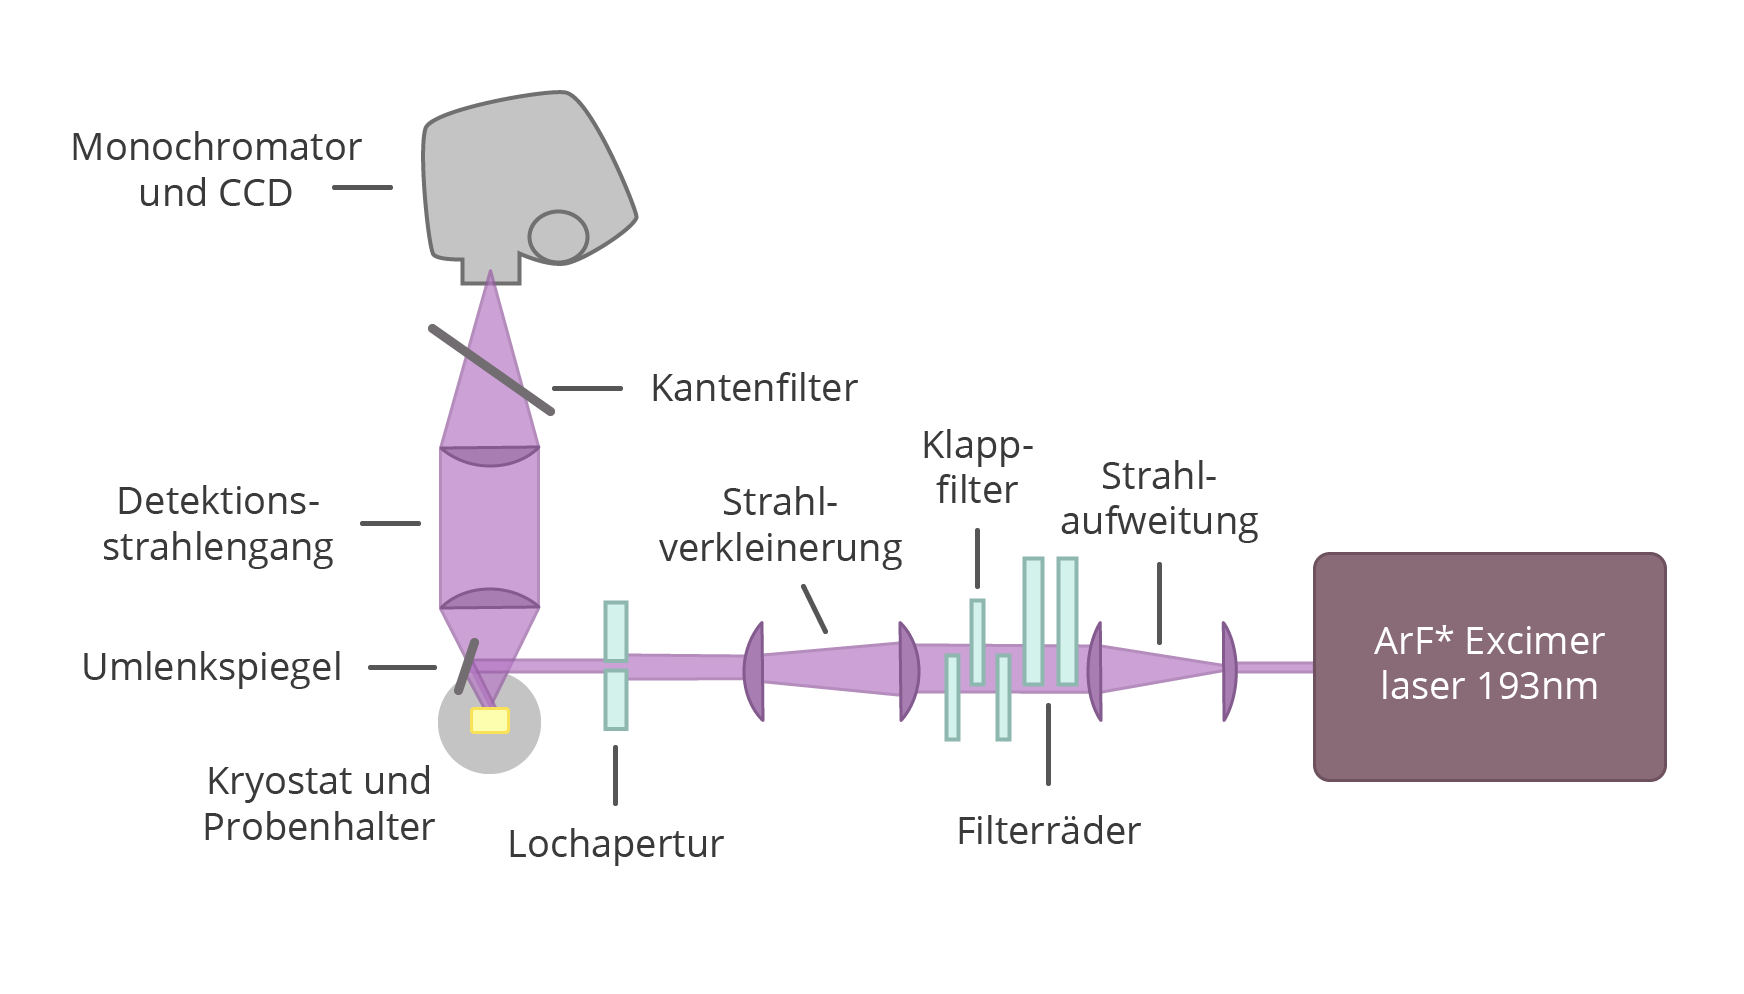
\includegraphics[width=0.9\linewidth]{Bilder/aufbauPL.png}
        \caption{}
        \label{fig:wurtz}
    \end{minipage}% <- sonst wird hier ein Leerzeichen eingefügt
\end{figure}
\vspace{1cm}
\raggedright

Für die experimentelle Untersuchung der UV-Photolumineszenz wurde der PL-Aufbau der AG-Kneissl verwendet, den Christoph Reich in der Zeit seiner Masterarbeit aufgebaut und während seiner Promotion erweitert hat~\cite{creich}. 
Als Anregungsquelle für die Photolumineszenz dient ein ArF-Excimerlaser mit einer Wellenlänge von $193 \ nm$ ($6,4 \ eV$). Mit dieser Wellenlänge ist er bestens geeignet für die Überbandanregung von Nitridhalbleitern. 
Des Weiteren bietet der Aufbau die Möglichkeit von temperaturabhängigen Untersuchungen von $5 \ K $ bis $300 K$. Dies ist auch die Grundlage für die Bestimmung der Internen Quanteneffizienz (kurz IQE), die den Großteil der Thematik dieser Arbeit ausmachen wird. 
\newline
Der Laser mit dem Modellnamen  "Xantos" von der Firma Coherent bietet eine maximale Emissionsenergie von $ 5 \ mJ $ und die Frequenz ist bis zu 500 Hz einstellbar bei einer Pulsdauer von $5 \ ns$. 
Durch interne Rückkopplung ist eine Energiestabilisierung möglich, die die Schwankung der Anregungsleistung auf 3 Prozent minimiert. 
\newline
Die Ansteuerung des kompletten Messvorgangs erfolgt durch die Messsoftware von Christoph Reich, entwickelt in der grafischen Programmiersprache "LabView" von Texas Instruments. Mit dieser ist es möglich alle nötigen Einstellungen an Pumpen, Heizern, Laser, Filtern und Spektrometer vorzunehmen, um einen komplett automatisierten Messvorgang zu starten, der nur noch aus Sicherheitsbedingungen überwacht werden muss. Spektren können so mit verschiedenen Parametern wie Position, Anregungsleistungsdichte, Temperatur, Energiebereich und Integrationszeit aufgenommen werden und auch ein Gaswechsel ist möglich.
\newline
Beginnend vom Laser wird im ersten Schritt der Lasterstrahl durch ein Linsensystem bestehend aus einer Zerstreuungs- und Sammellinse aufgeweitet. Dieser Schritt ermöglicht es, die Anregungsleistungsdichte zu verringern, um die am Aufbau beteiligten Gerätschaften nicht mit zu hohen Leistungen zu beschädigen. Damit sind insbesondere die Filterräder gemeint. Mit Hilfe der Filterräder ist es möglich, die Anregungsleistungsdichte 61 stufig zu variieren und somit leistungsdichteabhängige IQE Messungen zu machen. Als nächstes passiert der Strahl ein Linsensystem aus zwei Sammellinsen für eine Strahlverkleinerung. Vor dem Auftreffen des Strahles am Probenhalter im Kryostaten passiert der Strahl noch eine Lochblende. Sie dient der Entfernung achsennaher Strahlen und um bei Bedarf den Strahldruchmesser noch weiter zu verringern. Um den Strahl in Richtung des Probenhalters durch das Fenster im Kryostaten zu lenken, wird ein Spiegel mit einer dielektrischen Beschichtung benutzt. Der Laserstrahl durchdringt die Fenster des Kryostaten, diese sind speziell für eine hohe Transmission in diesem Wellenlängenbereich ausgelegt. Der Kryostat selbst ist horizontal und vertikal verfahrbar um die Messung mehrerer Proben im Probenhalter in einem Vorgang zu ermöglichen. Die Proben werden mit einem Kleber auf dem Probenhalter selbst befestigt, bevor dieser in den Kryostaten geschoben wird. 
Die Anregung der Proben mit dem Laserstrahl führt zur Proben spezifischen Emission von Licht. Diese wird von einer Linse im Strahlengang vor dem Detektor eingefangen und von einer zweiten Linse eingefangen die auf den Monochromatorspalt fokussiert ist.

